
\subsection{How do skilled performers perform better on flat section in slalom?}


\subsubsection{Which strategies are best to perform well on flats?}
We began by studying which technical strategies enable skilled alpine skiers to descend a flat slalom course as quickly as possible. The strategies we examined in study 3 were "stand against," "rock skis forward," "extend," and "extend with rock skis forward." We began testing after a familiarizing session where we introduced skiers to the strategies and allowed them to practice until they understood and mastered the techniques. Once understood, the skiers performed a total of eight trials (two on each strategy) that were randomly assigned to each skier under the condition that the first and last four trials included all four strategies. Therefore, we could use the data to estimate which technical strategies enable skilled alpine skiers to descend a flat slalom course as quickly as possible.

We employed a Bayesian modeling approach (model 1) to estimate the differences between the strategies. The analysis revealed that skiers on average achieved their best descent times using the 'extend with rock skis forward' strategy (16.66, 95\% credible interval (CI) = 16.54, 16.77). The second best strategy for skiers was to step down to solely "extend," which was only 0.02 sec. (95\% CI = -0.02, 0.06) slower than the "extend with rock skis forward" strategy. However, when skiers switched from the "extend" strategy to the "rock ski forward" strategy, the expected time loss was 0.21 sec. (95\% CI = 0.16, 0.25). Finally, if the skiers switched from the "rock skis forward" strategy to the "stand against" strategy, the expected time loss was 0.2 sec. (95\% CI = 0.15, 0.25). Therefore, the strategies the skiers used made a great difference in race time.

The results show that just skiing cleanly and resisting centripetal forces during a turn does not suffice to achieve fast race times on flat terrain in slaloms. Instead, the active movements of the skiers were crucial for achieving good race times on flats. "Rock skis forward" resulted in significant improvements in race times compared to 'stand against'. This finding aligns well with prior findings in slalom skiing, showing a strong correlation between fore and aft movements and energy dissipation, such that more fore movements are associated with greater energy dissipation \cite{reid_turn_2009, reid_kinematic_2010}. Furthermore, studies have shown that faster skiers have a greater range of fore/aft motion and spend a larger portion of the turn skiing with their weight shifted back after gate passage than slower skiers \cite{tjorhom_beskrivelse_2007, reid_kinematic_2010}. Our results extend these findings and provide experimental evidence that "rock skis forward" can be an effective strategy for improving race times on flat terrain in slalom.

The 'rock skis forward' strategy resulted in much slower times than did the 'extend' strategy, however. Predictions from the Lind and Sanders model \cite{lind_physics_2013} indicate that extending the center of mass closer to the axis of rotation during a turn from a laterally inclined position should significantly improve the race time. Without motion capture data, we cannot assess the extent to which skiers extended and the resulting increase in kinetic energy. Nonetheless, the results suggest that skiers' extension movements play a crucial role in slalom performance, contrary to previous claims \cite{supej_differential_2008}.

Finally, we found that "extend with rock skis forward" on average was the best strategy. This finding aligns with previous simulations suggesting that this strategy is most effective when skiers pump over rollers \cite{mote_accelerations_1983} and that it can be transferred to skiers executing a turn \cite{reid_kinematic_2010}. However, it is important to emphasize that "extend with rock skis forward" only was marginally better than the "stretching" strategy alone. One reason for the limited improvement achieved by adding "rock skis forward" to the "extend" strategy might be that rocking the skis forward during the turn compromised how much the skier could extend toward the turn's axis of rotation. For instance, extensive extension could be challenging if the skier's center of mass was located at the tail of the skis. This issue should be further investigated in future analyses.

One limitation of these timing analyses is that we do not have precise knowledge of how much the skiers moved when executing the strategies or how these strategies affected the mechanical energy during a turn. Therefore, we cannot comment on the skiers' actual execution or the energy mechanics behind each strategy. Future studies should incorporate motion capture to address this gap in understanding.



\begin{figure}[H]
\centering
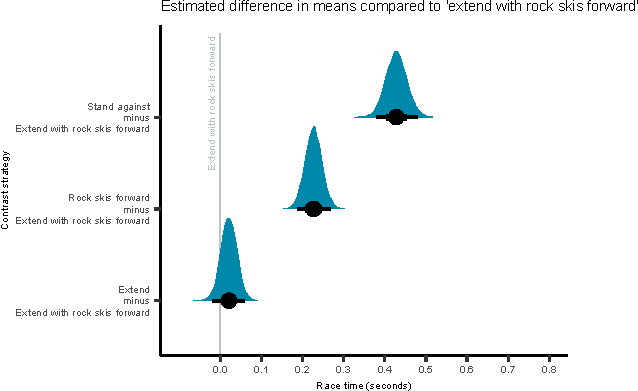
\includegraphics{figure_results_Q1_strategies.pdf}
\caption{Estimated differences in means compared to 'extend with rock skis forward'. The circle represents the point estimates whereas the shaded distribution represents the posterior distribution fitted from the model}
\label{fig:q1_strategieseffect}
\end{figure}



Velocity}
We found that the skiers improved their race times in both the intermediate split and the local positioning sections, which inspired us to continue studying the kinematic changes among skiers in the local positioning section. If the improvement in the skiers' race times can be attributed to the pumping mechanism, we would expect skiers to increase their velocity around or immediately after gate passage, at the time when the extension movement occurs.  Figure \ref{fig: velocity}a shows the velocity profiles for the local positioning system section during baseline and retention. We first describe the global velocity trend at baseline and then the contrast between baseline and retention.

Before the intervention (baseline), the skiers' velocity nearly declined for every gate in the local positioning sequence compared to their velocity during straight gliding. With the exception of a slight velocity increase of 0.05 m/s (95\% CI [-0.08, 0.17]) from gate 1 to gate 2, the velocities decreased on average by -0.06 m/s (95\% CI [-0.19, 0.07]) from gate 2 to gate 3 and by -0.12 m/s (95\% CI [-0.25, 0]) from gate 3 to gate 4 compared to straight gliding times. We focused only on comparisons at the gates because the gates mark a fixed reference point. 

After the training intervention, skiers increased their entry velocity into the local positioning section (gate 1) by an average of 0.24 m/s (95\% CI [0.19, 0.29]) compared to the baseline velocity. However, the skiers also tended to increase their velocity throughout the section. Specifically, the skiers increased their velocity on average by 0.07 m/s (95\% CI [0.01, 0.12]) from gate 1 to gate 2, followed by a slight decrease of -0.02 m/s (95\% CI [-0.05, 0.02]) from gate 2 to gate 3. Subsequently, the velocity of the skiers increased again by 0.1 m/s (95\% CI [0.06, 0.14]). Therefore, the velocity of the skiers increased almost incrementally from gate to gate. Besides, the velocity profiles appeared more wavy, as depicted in Fig. \ref{fig: velocity}b. In general, the pattern of these waveforms was that skiers increased their velocity after gate passage and continued to rise until the skier was between two gates. After that, the velocity decreased to the6 gate passage before it rose again. 

\begin{figure}[H]
\centering
\includegraphics{figurer/figure_velocity_3.pdf}
\caption{Velocity in the local positioning system section. \textbf{a.} Estimated velocity during baseline and retention for the local positioning section. \textbf{b}. Estimated differences (contrast) between baseline and retention for the local positioning section. The black lines denote the expected mean or differences in mean, with the shaded area representing their 95\% credible interval (CI). Each gray point or line represents one run trial by a skier}\label{fig: velocity}
\end{figure}

\subsection{Acceleration}
We continued examining acceleration through the turn to analyze the velocity changes more closely. As shown in Fig. \ref{fig: acc}a, the acceleration exhibited fluctuating waves, with skiers increasing their acceleration up to about the switch between two turns that began just before or around the gate passage. After this switch, the skiers decelerated until just before the gate. 

During the baseline, we found that the skiers' acceleration decreased on average by -0.91 m/s$^2$ (95\% CI [-1.71, -0.05]) from gate 1 to gate 2, followed by an increase of 0.42 m/s$^2$ (95\% CI [-0.40, 1.31]) from gate 2 to gate 3 and then a marginal increase of 0.01 m/s$^2$ (95\% CI [-0.84, 0.79]) again from gate 3 to gate 4, compared to the acceleration during straight gliding.

Following the intervention, the skiers developed a significantly more wavy acceleration profile with higher peaks and lower troughs compared to the baseline. We performed a gate-to-gate analysis, which revealed that acceleration was lower at gate 1 by -0.53  m/s$^2$ (95\% CI [-0.66, -0.41]), at gate 2 by -0.19  m/s$^2$ (95\% CI [-0.26, -0.13]), at gate 3 by -0.48  m/s$^2$ (95\% CI [-0.54, -0.42]), and at gate 4 by -0.42  m/s$^2$  (95\% CI [-0.48, -0.36]) compared to the baseline. Fig. \ref{fig: acc}b shows the expected mean difference between baseline and retention. 

To better understand how the acceleration changed between baseline and retention in each turn, we computed the total acceleration from gate to gate through the local positioning sequence. From this model, we found that the estimated difference in total acceleration was 24.4 (95\% CI [-14.4, 63.1]) from slalom gate 1 to slalom gate 2, 1.65 (95\% CI [-37.6, 40.1]) between gate 2 and gate 2, 39.4 (95\% CI [0.59, 78.1]) from gate 3 to gate 4, and 107.0 (95\% CI [68.8, 146.0]) from gate 4 to the end of the sequence. Therefore, the skiers appears to have had a positive overall acceleration in most of the gates in the sequence. Fig. \ref{fig: acc}c and d show the total acceleration during each gate in the local positioning section.

\begin{figure}[H]
\centering
\includegraphics{figurer/figure_acc_2.pdf}
\caption{Acceleration in the local positioning system section.\textbf{a.} Estimated acceleration during baseline and retention for the local positioning section. \textbf{b}. Expected mean difference between baseline and retention in the local positioning section.\textbf{c.} Estimated total gate-to-gate acceleration during baseline and retention in the local positioning section. \textbf{d}. Expected mean difference between baseline and retention in the local positioning section. The black lines denote the expected mean or differences in mean, with the shaded area representing their 95\% credible interval (CI). Each gray point or line represents one run trial by a skier}\label{fig: acc}
\end{figure}

\subsection{Path length}
Finally, we analyzed the path length, which we expected not to undergo massive changes according to our measurements from the local positioning system. In the case of change, we would expect it to be shorter during retention than during baseline because skiers (theoretically) would ski a shorter path length as they extended toward the axis of rotation during the turn.

At baseline, we found that the total path length from gate 1 to gate 2 was 91.53 (95\% CI [83.86, 99.30]), 92.57 (95\% CI [84.75, 100.45]) from gate 2 to gate 3, and 87.30 (95\% CI [79.40, 95.32]) from gate 3 to gate 4, while it was 69.30 (95\% CI [61.35, 77.16]) from gate 4 to the end of the section. Notably, the reason for the lower estimate from gate 4 to the end is that this section was shorter than the other sections. Fig. \ref{fig: path}a shows the total path length during each gate in the local positioning section.

\begin{figure}[H]
\centering
\includegraphics{figurer/figure_path.pdf}
\caption{Total path length in the local positioning system section.\textbf{a.} Estimated total path length during baseline and retention for the local positioning section. \textbf{b}. Expected mean difference in total path length between baseline and retention in the local positioning section. The black lines denote the expected mean or differences in mean, with the shaded area representing their 95\% credible interval (CI). Each gray point or line represents one run trial by a skier}\label{fig: path}
\end{figure}

As expected, we found only marginal differences between baseline and retention in total path length. The expected mean difference was -2.73 (95\% CI [-13.8, 8.23]) from gate 1 to gate 2, -2.08 (95\% CI [-12.9, 8.99]) from gate 2 to gate 3, and -1.99 (95\% CI [-13.3, 9.18]) from gate 3 to gate 4, while it was -1.4 (95\% CI [-12.3, 9.62]) from gate 4 to the end of the section. Thus, there was considerable overlap in the expected differences in the mean difference in total path length. Fig. \ref{fig: path}b shows the expected mean difference in total path length during each gate in the local positioning section.